\documentclass[12pt]{article}
\setcounter{tocdepth}{4}
 \setcounter{secnumdepth}{4}
\renewcommand{\labelenumii}{\theenumii}
\renewcommand{\theenumii}{\theenumi.\arabic{enumii}.}
\usepackage[utf8]{inputenc}
%\usepackage[T1]{fontenc}

\usepackage{geometry}
\geometry{a4paper}
\usepackage{graphicx}
\usepackage{float}
\usepackage[italian]{babel}

\linespread{1.2}
\setlength{\parindent}{0pt}

\usepackage[T1]{fontenc}
\usepackage{inconsolata}

\usepackage{color}
\definecolor{bluekeywords}{rgb}{0.13,0.13,1}
\definecolor{greencomments}{rgb}{0,0.5,0}
\definecolor{redstrings}{rgb}{0.9,0,0}

\usepackage{listings}
\lstset{language=[Sharp]C,
  showspaces=false,
  showtabs=false,
  breaklines=true,
  showstringspaces=false,
  breakatwhitespace=true,
  escapeinside={(*@}{@*)},
  commentstyle=\color{greencomments},
  keywordstyle=\color{bluekeywords},
  stringstyle=\color{redstrings},
  basicstyle={\footnotesize\ttfamily},   
}


\definecolor{lightgray}{rgb}{0.95, 0.95, 0.95}
\definecolor{darkgray}{rgb}{0.4, 0.4, 0.4}
%\definecolor{purple}{rgb}{0.65, 0.12, 0.82}
\definecolor{editorGray}{rgb}{0.95, 0.95, 0.95}
\definecolor{editorOcher}{rgb}{1, 0.5, 0} % #FF7F00 -> rgb(239, 169, 0)
\definecolor{editorGreen}{rgb}{0, 0.5, 0} % #007C00 -> rgb(0, 124, 0)
\definecolor{orange}{rgb}{1,0.45,0.13}		
\definecolor{olive}{rgb}{0.17,0.59,0.20}
\definecolor{brown}{rgb}{0.69,0.31,0.31}
\definecolor{purple}{rgb}{0.38,0.18,0.81}
\definecolor{lightblue}{rgb}{0.1,0.57,0.7}
\definecolor{lightred}{rgb}{1,0.4,0.5}
\usepackage{upquote}
\usepackage{listings}
% CSS
\lstdefinelanguage{CSS}{
  keywords={color,background-image:,margin,padding,font,weight,display,position,top,left,right,bottom,list,style,border,size,white,space,min,width, transition:, transform:, transition-property, transition-duration, transition-timing-function},	
  sensitive=true,
  morecomment=[l]{//},
  morecomment=[s]{/*}{*/},
  morestring=[b]',
  morestring=[b]",
  alsoletter={:},
  alsodigit={-}
}

% JavaScript
\lstdefinelanguage{JavaScript}{
  morekeywords={typeof, new, true, false, catch, function, return, null, catch, switch, var, if, in, while, do, else, case, break},
  morecomment=[s]{/*}{*/},
  morecomment=[l]//,
  morestring=[b]",
  morestring=[b]'
}

\lstdefinelanguage{HTML5}{
  language=html,
  sensitive=true,	
  alsoletter={<>=-},	
  morecomment=[s]{<!-}{-->},
  tag=[s],
  otherkeywords={
  % General
  >,
  % Standard tags
	<!DOCTYPE,
  </html, <html, <head, <title, </title, <style, </style, <link, </head, <meta, />,
<agm-info-window, </agm-info-window, <agm-marker, </agm-marker, <agm-map, </agm-map, <app-marker-detail, </app-marker-detail
	% body
	</body, <body,
	% Divs
	</div, <div, </div>, 
	% Paragraphs
	</p, <p, </p>,
	% scripts
	</script, <script,
  % More tags...
  <canvas, /canvas>, <svg, <rect, <animateTransform, </rect>, </svg>, <video, <source, <iframe, </iframe>, </video>, <image, </image>, <header, </header, <article, </article
  },
  ndkeywords={
  % General
  =,
  % HTML attributes
  charset=, src=, id=, width=, height=, style=, type=, rel=, href=, latitude=, longitude=
  % SVG attributes
  fill=, attributeName=, begin=, dur=, from=, to=, poster=, controls=, x=, y=, repeatCount=, xlink:href=,
  % properties
  margin:, padding:, background-image:, border:, top:, left:, position:, width:, height:, margin-top:, margin-bottom:, font-size:, line-height:,
	% CSS3 properties
  transform:, -moz-transform:, -webkit-transform:,
  animation:, -webkit-animation:,
  transition:,  transition-duration:, transition-property:, transition-timing-function:,
  }
}

\lstdefinestyle{htmlcssjs} {%
  % General design
%  backgroundcolor=\color{editorGray},
  basicstyle={\footnotesize\ttfamily},   
  % line-numbers
  % Code design
  identifierstyle=\color{black},
  keywordstyle=\color{blue}\bfseries,
  ndkeywordstyle=\color{editorGreen}\bfseries,
  stringstyle=\color{editorOcher}\ttfamily,
  commentstyle=\color{brown}\ttfamily,
  % Code
  language=HTML5,
  alsolanguage=JavaScript,
  alsodigit={.:;},	
  tabsize=2,
  showtabs=false,
  showspaces=false,
  showstringspaces=false,
  extendedchars=true,
  breaklines=true,
}
%
\lstdefinestyle{py} {%
language=python,
literate=%
*{0}{{{\color{lightred}0}}}1
{1}{{{\color{lightred}1}}}1
{2}{{{\color{lightred}2}}}1
{3}{{{\color{lightred}3}}}1
{4}{{{\color{lightred}4}}}1
{5}{{{\color{lightred}5}}}1
{6}{{{\color{lightred}6}}}1
{7}{{{\color{lightred}7}}}1
{8}{{{\color{lightred}8}}}1
{9}{{{\color{lightred}9}}}1,
basicstyle=\footnotesize\ttfamily, % Standardschrift
numbers=left,               % Ort der Zeilennummern
%numberstyle=\tiny,          % Stil der Zeilennummern
%stepnumber=2,               % Abstand zwischen den Zeilennummern
numbersep=5pt,              % Abstand der Nummern zum Text
tabsize=4,                  % Groesse von Tabs
extendedchars=true,         %
breaklines=true,            % Zeilen werden Umgebrochen
keywordstyle=\color{blue}\bfseries,
frame=b,
commentstyle=\color{brown}\itshape,
stringstyle=\color{editorOcher}\ttfamily, % Farbe der String
showspaces=false,           % Leerzeichen anzeigen ?
showtabs=false,             % Tabs anzeigen ?
xleftmargin=17pt,
framexleftmargin=17pt,
framexrightmargin=5pt,
framexbottommargin=4pt,
%backgroundcolor=\color{lightgray},
showstringspaces=false,      % Leerzeichen in Strings anzeigen ?
}%
%


\begin{document}

%----------------------------------------------------------------------------------------
%	TITOLO
%----------------------------------------------------------------------------------------

\begin{titlepage}

\newcommand{\HRule}{\rule{\linewidth}{0.5mm}}

\center

\textsc{\Large Relazione di progetto di "Smart City e Tecnologie Mobili"}\\[0.5cm]

\HRule \\[0.4cm]
{ \huge \bfseries Smart Public Restroom }\\[0.4cm]
\HRule \\[1.5cm]

\vfill

\begin{flushleft}
\emph{Numero del gruppo:}\\[1cm]
\emph{Componenti del gruppo:}\\[3cm]
\end{flushleft}



\end{titlepage}

%----------------------------------------------------------------------------------------
%	INDICE
%----------------------------------------------------------------------------------------

\tableofcontents

\newpage

%----------------------------------------------------------------------------------------
%	INTRODUZIONE
%----------------------------------------------------------------------------------------

\section{Introduzione}

Esporre l’obiettivo del progetto dandone una visione complessiva.\\

Devono essere illustrate le caratteristiche salienti del progetto; deve essere chiara la distinzione tra le tecnologie usate/assemblate durante lo svolgimento dell'elaborato e il contributo tecnologico/scientifico effettivamente apportato dal gruppo.\\


Vincoli circa la lunghezza della sezione (escluse didascalie, tabelle, testo nelle immagini, schemi):

\vspace{1cm}
\begin{tabular}{l|rr}
 & Numero minimo di battute & Numero massimo di battute \\
 \hline
 1 componente & 2000 & 3000 \\
 2 componenti & 2500 & 4500 \\
 3 componenti & 3000 & 6000 \\
 \hline
\end{tabular}


\newpage


%----------------------------------------------------------------------------------------
%	STATO DELL'ARTE
%----------------------------------------------------------------------------------------

\section{Stato dell'arte}

Riassumere le soluzioni presenti in letteratura inerenti al problema in esame. Per ciascuna, discutere le principali diversità o affinità rispetto al progetto presentato. Nel caso non siano presenti soluzioni direttamente comparabili a quella presentata descrivere comunque le principali tecniche note per affrontare la tematica trattata.\\

Le soluzioni esposte devono essere corredate degli opportuni riferimenti bibliografici. Nel caso si tratti di soluzioni già operative sul mercato, devono essere indicate le fonti (online) dove poter accedere al servizio o approfondirne i contenuti.\\


Vincoli circa la lunghezza della sezione (escluse didascalie, tabelle, testo nelle immagini, schemi):

\vspace{1cm}
\begin{tabular}{l|rr}
 & Numero minimo di battute & Numero massimo di battute \\
 \hline
 1 componente & 2000 & 3000 \\
 2 componenti & 2500 & 4500 \\
 3 componenti & 3000 & 6000 \\
 \hline
\end{tabular}


\newpage


%----------------------------------------------------------------------------------------
%	ANALISI DEI REQUISITI
%----------------------------------------------------------------------------------------

\section{Analisi dei requisiti}
\subsection{Requisiti}

È necessario realizzare un sistema di gestione per bagni pubblici che consenta a un utente amministrativo, da remoto, di visionare lo stato generale di un impianto.\\
Nel dettaglio ci si aspetta che un utente possa, dato uno specifico impianto, visualizzare in tempo reale:
\begin{itemize}
\item Indicazioni sulla quantità di sapone per le mani rimasto in ogni dispenser, indicato in centesimi.
\item Indicazioni sul tasso di riempimento di ogni pattumiera presente, indicata in centesimi.
\item Indicazioni sullo stato aperto/chiuso di ogni singola cella dell'impianto.
\item Indicazioni sullo stato disponibile/terminata di ogni dispenser di carta igienica presente nelle celle dell'impianto.
\item Indicazioni sullo stato funzionante/non funzionante delle luci di cortesia ad ogni cella.
\item Indicazioni sul tasso di umidità di ogni cella dell'impianto.
\item Indicazioni su eventuale presenza di fumo.
\end{itemize}
Le informazioni sopra riportate dovranno essere visionabili attraverso un apposita app chiamata \textit{manager}, che fungerà da supporto gestionale dei bagni pubblici installati.\\
A fronte infatti di un semplice autenticazione tramite utente/password, infatti, l'app dovrà inoltre consentire di: 
\begin{itemize}
\item Aggiungere nuovi impianti al sistema.
\item Visualizzare e, all'occorrenza, modificare alcune informazioni di carattere generale sui bagni pubblici installati, come ad esempio indirizzo, coordinate GPS e azienda di manutenzione assegnata.
\item Aggiungere nuovi utenti di amministrazione.
\item Visualizzare eventuali report utente sullo stato del sistema dell'app \textit{consumer}.
\end{itemize}
Si dovrà anche fornire un apposita app (chiamata \textit{consumer}) a supporto di tutti i cittadini e turisti che si vogliono recare in un ambito pubblico in un certo momento della giornata.\\
L'app dovrà mostrare a schermo la locazione di ogni bagno pubblico (tramite \textit{markers} o simile) disponibile e, all'occorrenza, riportare lo stato degli stessi: qualora un bagno pubblico non sia agibile per qualche motivo, tale informazione dovrà essere opportunamente riportata.\\
Nel dettaglio, l'app \textit{consumer} dovrà consentire di:
\begin{itemize}
\item Visualizzare una \textit{gmap} (centrata sulla locazione corrente) con indicati i bagni pubblici disponibili del sistema.\\Ogni bagno, se selezionato, dovrà mostrare informazioni utili al cittadino circa il loro stato corrente.
\item Riportare direttamente dall'app di eventuali problemi dell'applicazione/dei bagni pubblici riscontrati.
\end{itemize}
\newpage
\subsection{Analisi dei requisiti}
\subsubsection{Glossario}

\begin{center}
    \begin{tabular}{ | l |  p{10cm} |}
    \hline
    \textbf{Name} & \textbf{Definition} \\ \hline
    Impianto & Struttura rappresentante un bagno pubblico, contenente una serie di celle individuali. Ogni impianto è comprensivo di lavabi, dispenser di sapone e pattumiere. \\ \hline
    Cella & Struttura rappresentante una singola unità per servizi igienici comprensiva di gabinetto, carta igienica e luce di cortesia. \\ \hline
    `Manager` web App & Applicazione di amministrazione impianti utilizzata per gestire l'insieme dei bagni pubblici registrati nel network.\\ \hline
    `Consumer` web App & App di supporto al cittadino per individuare il più vicino bagno pubblico e visionare il suo stato corrente.\\ \hline
    gmap & Mappa geolocalizzata 2D fornita gratuitamente da \textit{Google} e molto conosciuta tra gli utenti.\\ \hline
    marker & Marcatore 2D posizionato in coordinate precise della gmap per segnalare la presenza di un punto di interesse.\\ \hline
    Utente amministrativo & Utente adibito a compiti di amministrazione e gestione dei bagni pubblici registrati nella rete, attraverso la web app \textit{manager}.\\ \hline
    Utente consumer & Utente della web app \textit{consumer}. \\ \hline
    \end{tabular}
\end{center}	
\newpage
\subsubsection{Casi d'uso}

\begin{figure}[h!]
  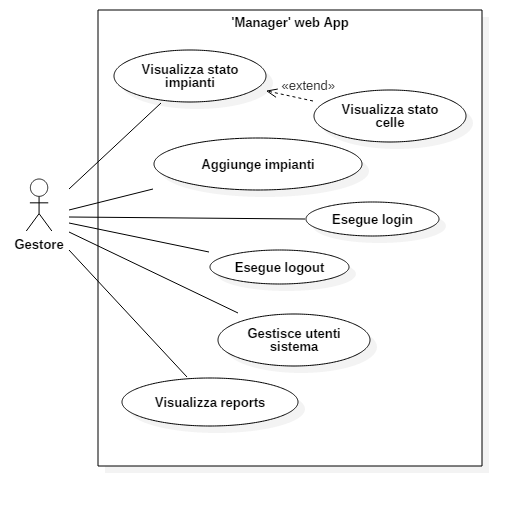
\includegraphics[scale=0.7]{img/usecase_manager.png}
  \caption{Casi d'uso per l'app `manager`}
  \label{fig:usecase_manager}
\end{figure}
\begin{figure}[h!]
  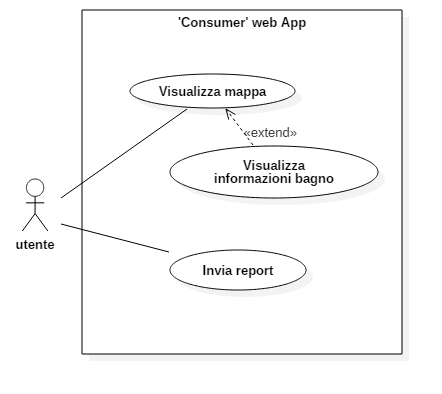
\includegraphics[scale=0.7]{img/usecase_consumer.png}
  \caption{Casi d'uso per l'app `consumer`}
  \label{fig:usecase_consumer}
\end{figure}
\newpage
\phantom{}
\newpage
\subsubsection{Requisiti funzionali}
\begin{enumerate}

\item Ogni sessione di utilizzo di \textit{manager} richiederà un autenticazione nella forma login/password.
\item Ogni impianto dovrà rendere disponibili i seguenti dati:
\begin{itemize}
\item Sapone residuo di ogni dispenser, espresso in centesimi.
\item Spazio residuo (tasso di riempimento) di ogni pattumiera, espresso in centesimi.
\item Eventuale presenza di fumo.
\end{itemize}
Per ogni cella saranno richiesti i seguenti dati:
\begin{itemize}
\item Segnalazione esaurimento carta igienica.
\item Stato di apertura della porta di accesso.
\item Tasso di umidità.
\item Segnalazione guasto luce di cortesia.
\end{itemize}
\item Gli utenti di \textit{manager} dovranno essere in grado di visualizzare i dati inviati dai sensori in tempo reale.
\item Dovrà essere possibile aggiungere nuovi impianti al sistema in qualsiasi momento.
\item Ogni impianto dovrà essere corredato dai seguenti dati:
\begin{itemize}
\item Indirizzo
\item Coordinate GPS
\item Azienda appaltratrice di manutenzione.
\end{itemize}
\item Ogni utente amministrativo di \textit{manager} dovrà essere in grado di creare nuovi utenti di amministrazione.
\item Ogni utente amministrativo di \textit{manager} dovrà essere in grado di visualizzare i reports utente sullo stato degli impianti o dell'app \textit{consumer}.
\item L'app \textit{consumer} dovrà adeguatamente funzionare su dispositivi mobili come smartphone e tablet con Android 8+ o iOS 11+.
\item L'app \textit{consumer}, all'avvio della gmap, dovrà centrarsi sulla posizione geolocalizzata del dispositivo.
\item La gmap di \textit{consumer} dovrà mostrare tutti gli impianti registrati nel sistema con appositi \textit{marker}.
\begin{enumerate}
\item Ogni impianto selezionato servirà per mostrare all'utente il suo stato corrente, con particolare attenzione circa la sua disponibilità.
\end{enumerate}
\item Ogni utente di \textit{consumer} potrà rilasciare, attraverso l'app, una segnalazione sullo stato dei servizi riscontrati.
\item \textit{consumer} dovrà essere nativamente installabile sul dispositivo dell'utente.
\end{enumerate}
\subsubsection{Requisiti non funzionali}
\begin{itemize}
\item \textbf{Dinamicità:} Il sistema dovrà consentire l’aggiunta e la rimozione di impianti sul territorio dinamicamente senza causare interruzioni generali del servizio.\\ Il sistema, pertanto, dovrà risultare adattabile ai cambiamenti della topologia di rete di cui è composto.
\item \textbf{Scalabilità:} Il sistema dovrà essere adattabile alla mole di informazioni inviata dagli impianti ed essere sufficientemente reattivo nei confronti delle richieste degli utenti, che aumenteranno gradualmente mano a mano che il sistema verrà adottato su tutto il territorio.\\
Verosimilmente, adottando il sistema su scala nazionale per i soli bagni pubblici, il numero di impianti da gestire si attesterà su qualche centinaio.\\
Anche considerando la partecipazione di bagni pubblici di natura privata (si pensi ai bagni degli autogrill), il numero totale di impianti non dovrebbe superare il migliaio di unità.\\ 
Il numero di utenti di amministrazione, considerati i punti sopra, dovrebbe rimanere pressoché trascurabile.\\
Gli utenti \textit{consumer}, d'altro canto, potranno raggiungere numeri considerevoli: particolare attenzione alla scalabilità dovrà essere riposta nello sviluppo dell'app per dispositivi mobili.
\item \textbf{Prestazioni:} Il sistema dovrà essere in grado di rispondere a tutte le richieste a cui andrà incontro con prestazioni ottimali, minimizzando il tempo di attesa di ogni azione intrapresa dagli utenti.\\
Dal punto di vista puramente applicativo, l'applicazione dovrà essere fluida nei caricamenti e nelle transizioni: ciò sarà possibile attraverso l'utilizzo di tecnologie all'avanguardia e restringendo il bacino di utenza dell'applicazione ai soli dispositivi più aggiornati.\\
Considerando la mole di dati coinvolta (e la loro non-criticità), si potrebbe considerare accettabile un aggiornamento dei valori di ogni impianto con intervalli di 10 secondi.
\item \textbf{Robustezza:} Il sistema dovrà offrire una buona tolleranza a tutti i guasti che si potranno presentare quotidianamente: errori di rete, anomalie delle letture dei sensori,  malfunzionamenti hardware ecc..\\ 
Gli eventuali malfunzionamenti riscontrati, infatti, non dovranno compromettere l'intero funzionamento del sistema ma soltanto le risorse direttamente collegate ad esso.\\ 
Eventuali fallimenti hardware (sia dei sensori che dei microcontrollori presenti) dovranno essere risolvibili sostituendo i singoli componenti difettosi, evitando così costose riconfigurazioni del sistema.\\
Qualora il server di sistema diventasse irraggiungibile, gli utenti \textit{consumer} dovranno comunque poter utilizzare l'app offline.

\item \textbf{Sicurezza:} Essendo le applicazioni esposte pubblicamente sulla rete, è importante che esse seguano i più elevati standard di sicurezza.\\
Tutte le applicazioni dovranno essere essere servite su HTTPS e protette da eventuali tentativi di attacco XSS da parte degli utenti.\\
Tutti gli accessi all'applicazione \textit{manager} (e, di conseguenza, al Database) necessiteranno di essere autenticati per limitare la superficie d'attacco di eventuali attori.\\
L'app consumer, venendo installata sul dispositivo degli utenti e possibilmente di milioni di persone, dovrà seguire i più elevati standard di sicurezza per evitare \textit{man-in-the-middle attacks} e qualsiasi uso non autorizzato dei servizi sopra descritti.

\item \textbf{Interoperabilità:} il sistema dovrà essere progettato per favorire il più possibile l'adozione di standard riconosciuti e, possibilmente, open-source.\\
In tal modo sarà possibile adattare il sistema a molteplici scenari e integrarlo con strumenti di terze parti, qualora lo si ritenga necessario.
\end{itemize}
%----------------------------------------------------------------------------------------
%	PROGETTAZIONE
%----------------------------------------------------------------------------------------
\newpage
\section{Progettazione}

Devono essere esposte le scelte progettuali operate nelle varie fasi di sviluppo dell'elaborato.\\

In questa sezione devono essere documentati gli schemi di progetto relativamente all'architettura complessiva del sistema e alle sue componenti di rilievo che possano meritare un'analisi di dettaglio. Per le componenti software si può ricorrere ad esempio a diagrammi delle classi, di sequenza, stato, attività. Per le componenti hardware è possibile includere opportuni schemi in grado di descrivere l'architettura fisica adottata.\\

Vincoli circa la lunghezza della sezione (escluse didascalie, tabelle, testo nelle immagini, schemi):

\vspace{1cm}
\begin{tabular}{l|rr}
 & Numero minimo di battute & Numero massimo di battute \\
 \hline
 1 componente & 9000 & 18000 \\
 2 componenti & 12000 & 21000 \\
 3 componenti & 15000 & 24000 \\
 \hline
\end{tabular}


\newpage
\subsection{Architettura del sistema}

Una breve analisi dei requisiti in un ottica progettuale ci porta a una suddivisione del sistema in tre parti logiche ben distinte: 
\begin{itemize}
	\item Una parte \textit{locale}, installata fisicamente in ogni impianto della rete, dedita alla raccolta di dati tramite sensori e al loro periodico invio.
	\\ Tutta l'insieme della componentistica hardware (e le relative problematiche) del progetto sarà concentrata in questa macro-area.
	\item Una parte \textit{applicativa}, dedita all'analisi dei dati raccolti, da parte di personale amministrativo e utenti \textit{consumer}.
	\item Una parte \textit{centrale}, costituita da un server (o, possibilmente, un insieme di server) dedita alla ricezione e archiviazione dei dati inviati dalle parti \textit{locali} del network.\\
	Questa entità si occuperà anche di distribuire le applicazioni (\textit{manager} e \textit{consumer}) agli utenti del sistema.
\end{itemize}

Una tale suddivisione del sistema consente di soddisfare pienamente i requisiti presentati nel capitolo precedente: la presenza di un \textit{middleware} (cioè il server)  tra le parti applicative e le parti locali consente di aumentare considerevolmente la sicurezza e la scalabilità dell'intero network.\\\\
La comunicazione tra la parte \textit{centrale} e parti \textit{applicative} e \textit{locali} avverrà tramite interfaccia RESTful, garantendo così i seguenti vantaggi:
\begin{itemize}
	\item \textit{Stateless}: non mantenendo su server alcuna informazione circa il contesto durante la connessione, ogni sessione utente è più sicura, performante e semplice.
	\item Compatibilità: essendo riconosciuto come standard \textit{de facto} nelle comunicazioni client-server (in virtù anche dei suoi requisiti meno stringenti rispetto ad altre forme di trasmissione formali come WSDL) è del tutto ragionevole considerare RESTFul un interfaccia applicabile in qualsiasi contesto di rete moderno.
	\item Affidabilità: una trasmissione RESTful JSON è composta sostanzialmente da una connessione HTTP tramite TCP/IP con un formato dati a bassissimo \textit{overhead}.\\
	Pertanto, ogni connessione si concluderà ad ogni singolo invio di dati:  ciò rende questa forma di comunicazione appetibile in contesti in cui non è possibile assicurare una connessione di rete stabile.
\end{itemize}
Viene riportato un diagramma dell'architettura logica della progettazione appena descritta:
\begin{figure}[h!]
\centering
  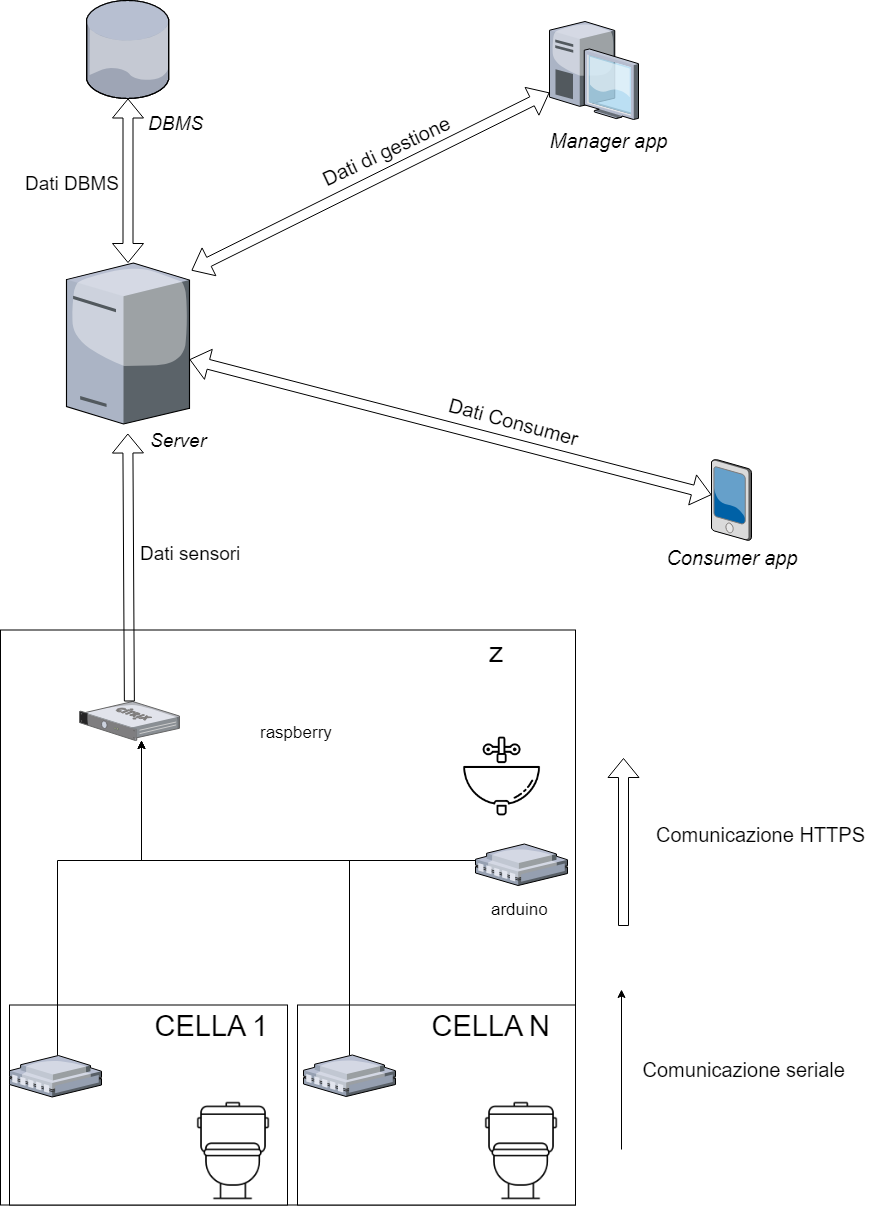
\includegraphics[scale=0.33]{img/architettura_logica-report.png}
  \caption{Architettura logica del sistema}
\end{figure}
\subsection{Progettazione parte locale}
Ogni parte \textit{locale} del sistema si occuperà di raccogliere i dati di utilizzo di ogni impianto (tramite l'utilizzo  
\newpage
\subsection{Progettazione parte applicativa}
Grazie all'analisi dei requisiti effettuata, si è evidenziato come il committente abbia richiesto la creazione di due applicazioni distinte, ognuna con una diversa finalità.\\
Purtroppo, ciò si scontra con la realtà del team di sviluppo incaricato alla produzione di \textit{manager} e \textit{consumer}: le risorse a disposizione sono piuttosto esigue, sia in termini di tempo che di manodopera.\\
Pertanto, come vedremo, verranno adottate strategie atte a ridurre i costi di sviluppo e rientrare, così, nel budget e nei tempi previsti.\\\\
Si tenga presente, inoltre, che data la loro reciproca indipendenza, ogni applicazione verrà analizzata separatamente nelle sottosezioni seguenti.
\subsubsection{Manager}
\paragraph{Ambiente}
I requisiti esposti dal committente riguardo la realizzazione di \textit{manager} non specificano il suo ambiente di utilizzo preferenziale: gli utenti potrebbero lavorare su macchine Windows o Linux indifferentemente.\\
A seguito di questa considerazione, e in relazione al fatto che non sono stati richieste funzionalità native specifiche di un qualche ambiente, si è deciso di realizzare \textit{manager} come \textit{web appplication}.\\
Tuttavia, sviluppare un'applicazione amministrativa per ambienti web  non consente soltanto di renderla pressoché universale, ma garantirà anche i seguenti benefici:
\begin{itemize}
\item Faciliterà la fase di distribuzione, in quanto non necessiterà di installazione locale (gli utenti potranno accedere all'applicazione attraverso un semplice browser web, che si presume già installato di default in tutti i sistemi operativi moderni).
 \item Renderà lo sviluppo della stessa più semplice, perché familiare all'insieme di skill pregresse del team di sviluppo.
\end{itemize}
Per rendere l'esperienza utente il più possibile vicina a una classica \textit{dekstop application} gestionale, \textit{manager} verrà sviluppata come una SPA (\textit{Single Page Application)}.\\\\
La decisione di sviluppare \textit{manager} per ambienti web, tuttavia, ha un costo ben definito in termini di compatibilità: il supporto ad alcune tecnologie per SPA, infatti, non potrà essere garantito  e ciò potrà portare ad escludere alcuni dispositivi particolarmente datati.
\paragraph{Autenticazione}
I requisiti esposti dal committente richiedono esplicitamente che gli utenti di amministrazione che utilizzano \textit{manager} debbano essere autenticati nel sistema, preferibilmente attraverso l'uso di username e password.\\
Data l'assenza di indicazioni in merito, il team di sviluppo si concentrerà solamente sulla realizzazione di autenticazioni con un singolo ruolo immutabile, ovvero quello di ``amministratore''; in altre parole, in questa prima iterazione del software qualsiasi utente connesso avrà pieno accesso a tutte le funzionalità del software.\\\\
Per evitare che ogni funzionalità ``protetta'' del prodotto richieda una forma di autenticazione all'utente, \textit{manager} utilizzerà un \textit{access token} scambiato dal server per ogni accesso successivo.\\
Tale \textit{access token} sarà costituito da una stringa casuale univoca e verrà salvato localmente nel browser utente: a tal scopo, esso verrà utilizzato come chiave di identificazione ad ogni successivo avvio dell'app, se presente.\\\\
È necessario tenere presente, tuttavia, che l'utilizzo di questo metodo di autenticazione non è esente da difetti o possibili rischi:
\begin{itemize}
\item Come qualsiasi altra risorsa locale salvata sul terminale utente, il \textit{loginToken} può essere accidentalmente (o volutamente) cancellato.\\ Purtroppo, questo rischio è particolarmente sentito in ambito web a causa alla relativa facilità con la quale è possibile cancellare la cache locale.
\item L'utilizzo di una chiave di accesso può esporre il sistema a rischi legati alla sicurezza: un terminale compromesso da un utente malintenzionato finirà infatti per esporre pubblicamente la propria chiave di accesso (attualmente, purtroppo, non vi è modo di archiviare in sicurezza le risorse locali di un browser).\\
Ottenuto così un \textit{loginToken} autentico, l'utente malintenzionato potrà effettuare attacchi \textit{masquerade} con la minima probabilità di essere scoperto.
\end{itemize}
Per rafforzare ulteriormente la sicurezza del sistema, inoltre, sarebbe opportuno associare un periodo di validità (ad esempio, 7 giorni) ad ogni \textit{loginToken}.\\
Qualora un utente non abbia effettuato l'accesso per un certo periodo prestabilito, infatti, la sessione sarà da riconvalidare con un nuovo accesso tramite i canali tradizionali.\\\\
Viene quindi presentato un breve diagramma di attività che riassume il funzionamento della login di \textit{manager}:
\begin{figure}[h!]
\centering
  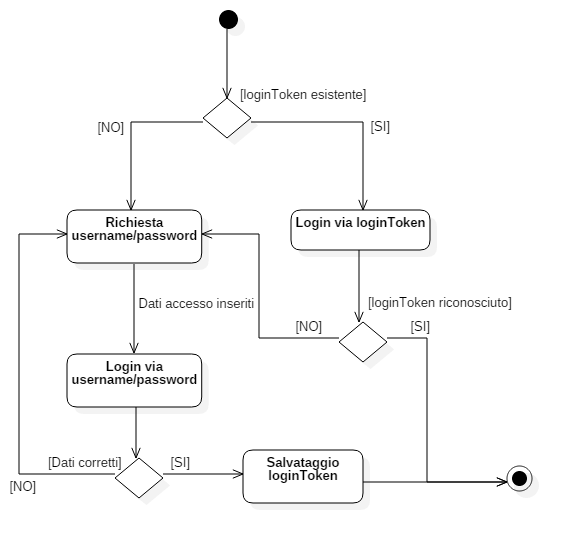
\includegraphics[scale=0.6]{img/activity_manager.png}
  \caption{Login \textit{manager}}
\end{figure}
\paragraph{Design}
Trattandosi di un applicazione di gestione e amministrazione, \textit{manager} non presenterà un'interfaccia ottimizzata per dispositivi mobile: si presume infatti che tutti gli utenti del sistema utilizzeranno il prodotto tramite uno schermo con sufficiente larghezza (ad esempio tramite un PC Fisso).\\Per questo motivo, il design si è incentrato su un interfaccia tipica per dispositivi desktop, come evidenziabile dal mockup seguente: 
\begin{figure}[h!]
\centering
  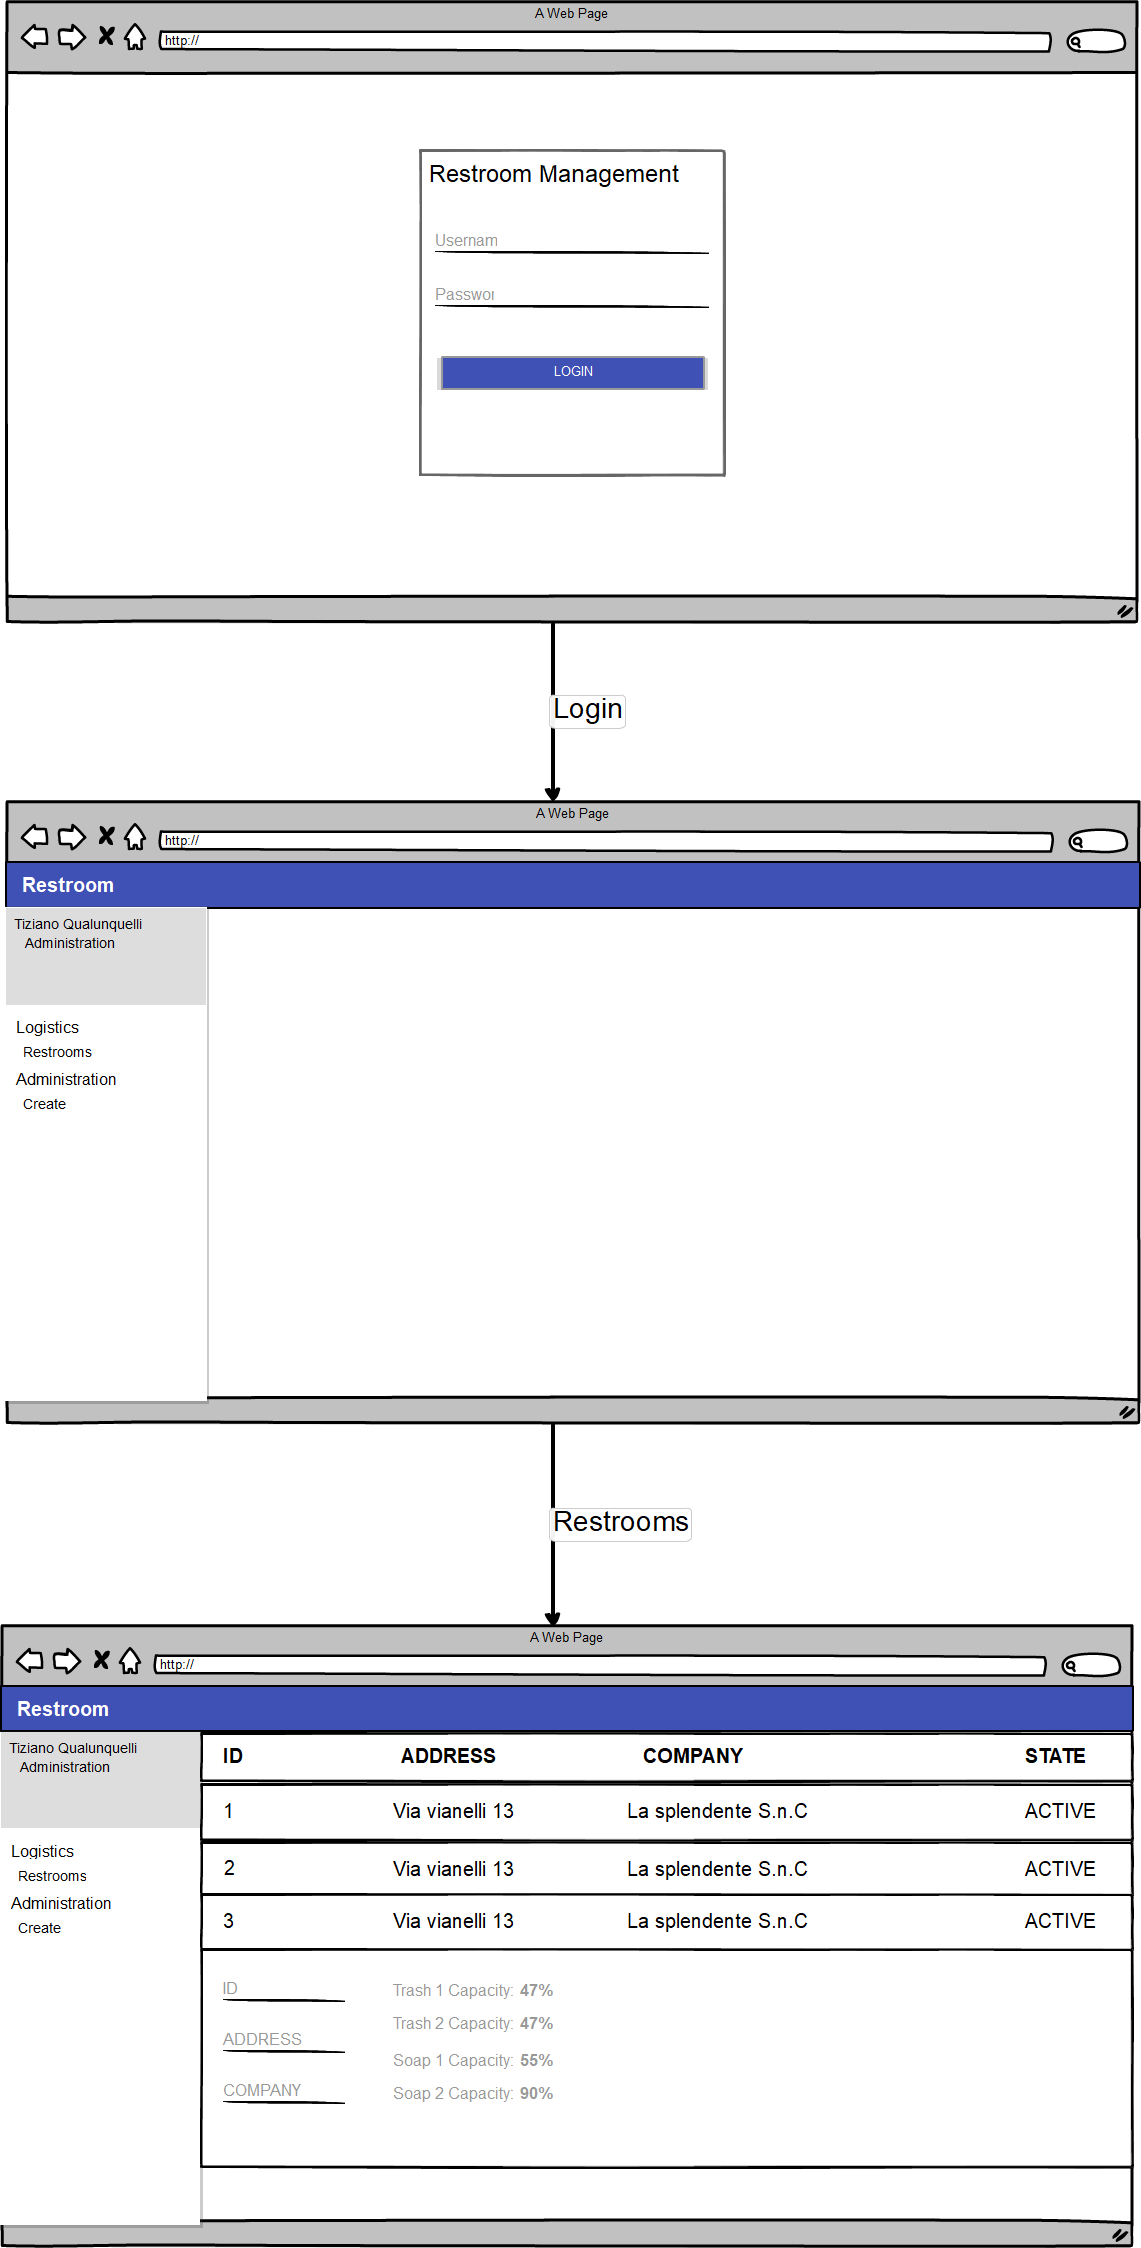
\includegraphics[scale=0.20]{img/mockup-manager.png}
  \caption{Mockup di \textit{manager}}
\end{figure}\\
A causa di una relativa familiarità a riguardo, il team di sviluppo si dedicherà ad uno stile \textit{Material Design} per tutte le schermate dell'applicazione.
\newpage
\subsubsection{Consumer}
\paragraph{Ambiente}
I requisiti esposti dal committente suggeriscono che \textit{consumer} debba essere un applicazione a larga diffusione, facile da utilizzare e performante; in altre parole, un applicazione il cui utilizzo da un grande numero di persone (come cittadini e turisti) sia fondamentale.\\
Questa considerazione porta all'adozione di esperienze utente (UX) e soluzioni popolari, atte a non scoraggiare l'utente finale dall'utilizzo di \textit{consumer} a causa di un eccessiva complessità; considerato inoltre che l'applicazione sarebbe indirizzata all'utilizzo anche da parte di turisti, il team di sviluppo si adopererà per lo sviluppo di una \textit{mobile application}.\\
Tuttavia, ciò comporterebbe una lievitazione considerevole dei costi di sviluppo: seppur ridotta in termini di funzionalità, sarebbe necessario infatti sviluppare un applicazione per ogni sistema operativo \textit{mobile} presente sul mercato (\textit{Android} e \textit{iOS}).\\\\
A seguito di tali considerazioni, si è deciso di sviluppare \textit{consumer} come PWA (\textit{Progressive Web App}) garantendo così i seguenti vantaggi:
\begin{itemize}
\item Sviluppo multipiattaforma: essendo sostanzialmente un'applicazione web di nuova concezione con specifiche ottimizzazioni per il mondo mobile, una PWA è naturalmente multipiattaforma (è soltanto necessario un browser aggiornato per il suo utilizzo).\\
Questa caratteristica aiuterà a contenere i costi di sviluppo, in quanto sarà necessario sviluppare soltanto un'applicazione per tutti gli ambienti.
\item Distribuzione svincolata: applicazioni di questo genere permettono di essere installate localmente sul dispositivo, scaricando tutti le dipendenze richieste al loro funzionamento.\\%imitando in tutto e per tutto il comportamento delle più classiche app native distribuite attraverso \textit{store}.\\
Ciò permette di garantire all'utente una UX da applicazione nativa, pur rimanendo distribuita attraverso un semplice URL: una caratteristica senza dubbio utile per evitare tutti i vincoli dei tradizionali canali di distribuzione delle app (come gli \textit{store}).
\item Familiarità: come per \textit{manager}, le scelte progettuali di \textit{consumer} sono state parzialmente influenzate dallo \textit{skill set} preesistente del team di sviluppo. 
\end{itemize}
Come per l'applicazione di amministrazione, tuttavia, emergono delle problematiche relative alle tecnologie supportate dai dispositivi per la PWA: alcuni device infatti potrebbero rivelarsi incompatibili perché troppo datati.\\
Benché questo aspetto vada chiaramente in contrasto con la necessità di rendere \textit{consumer} utilizzata da un gran numero di utenti, i requisiti funzionali richiesti dal committente saranno comunque rispettati nella loro totalità.\\
L'applicazione sarà comunque utilizzabile come un normale sito web: soltanto alcuni aspetti avanzati come l'installazione nativa, infatti, potranno risultare incompatibili.\newpage
\paragraph{Design}
La progettazione grafica di \textit{consumer} si è esclusivamente incentrata sulla creazione di un'app per dispositivi mobili incentrata sulla semplicità e immediatezza.\\
Per il prodotto non sono state infatti previste versioni specificatamente studiate per PC desktop: considerato che la mobilità è un requisito fondamentale per il committente, si può dire che il suo utilizzo attraverso un personal computer sia quanto meno scoraggiato.\\
A causa della sua maggiore popolarità nel settore mobile verrà utilizzato uno stile \textit{Material Design} per tutte le schermate del prodotto; ciò aiuterà ad orientare meglio l'utente al primo approccio in quanto ricalcherà pattern oramai universali.
Di seguito viene presentato un primo mockup coerente con i punti precedentemente esposti:
\begin{figure}[h!]
\centering
  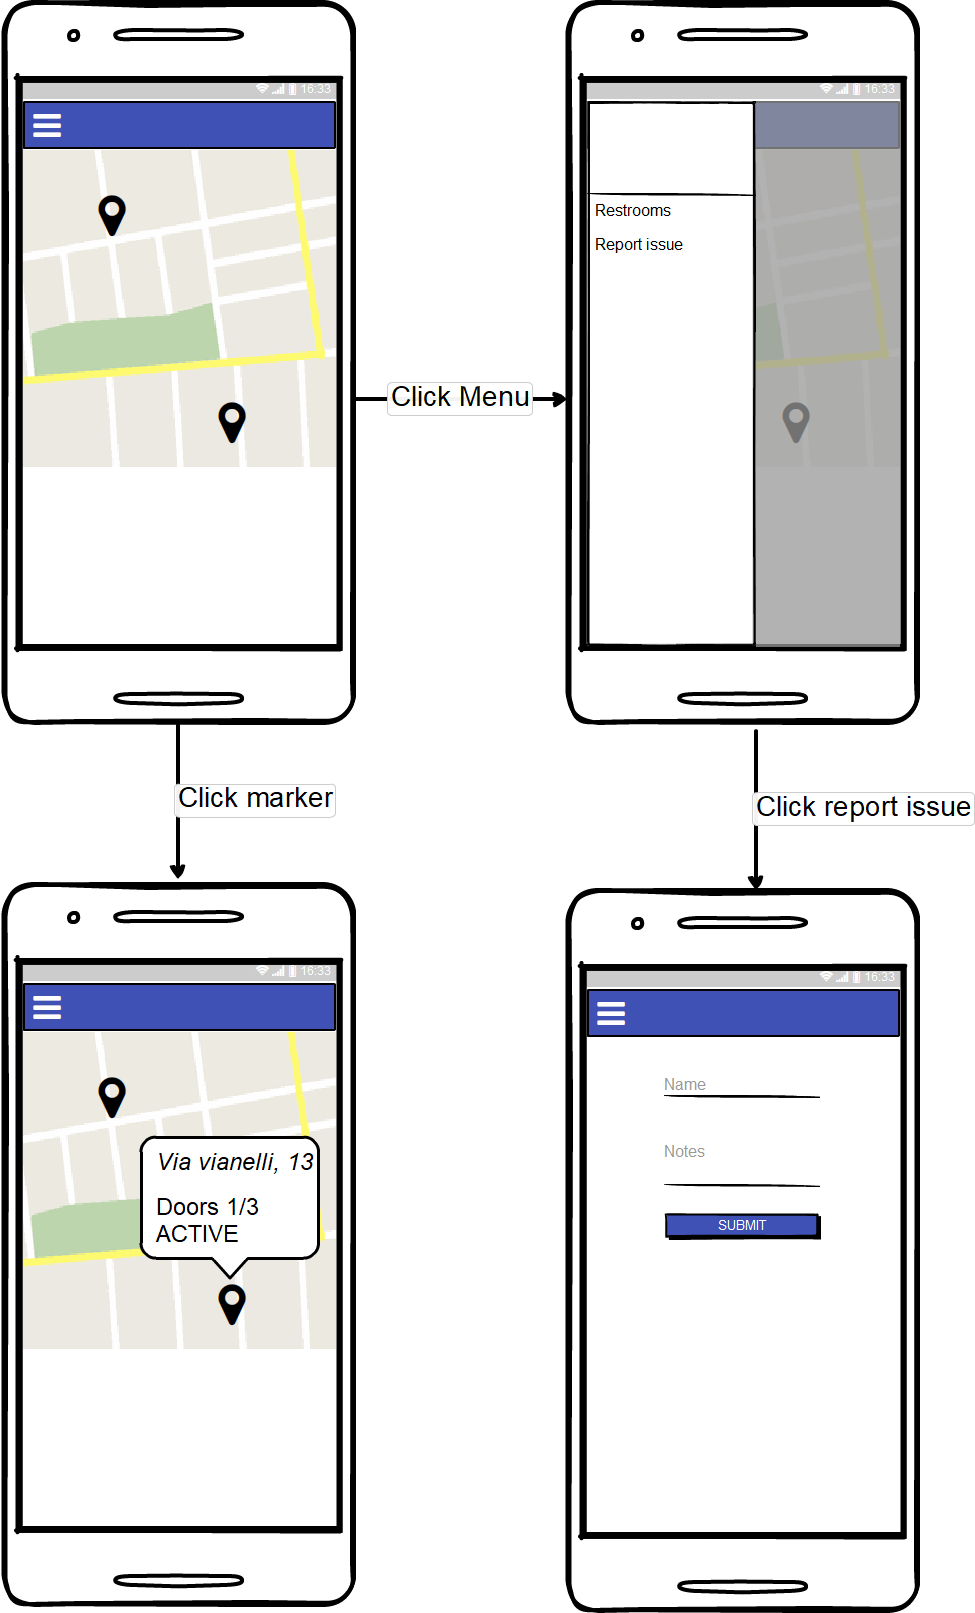
\includegraphics[scale=0.21]{img/mockup-consumer.png}
  \caption{Mockup di \textit{consumer}}
\end{figure}
\newpage
\subsection{Progettazione parte centrale}
La sezione di analisi dell'architettura ha evidenziato la necessità di creare un apposito \textit{server} RESTFul capace di fornire i dati richiesti dalle due applicazioni frontend (\textit{consumer} e \textit{manager}) e di raccogliere (e immagazzinare) i dati inviati dai singoli impianti installati.\\
Tali considerazioni profilano la realizzazione di 4 differenti entità:
\begin{itemize}
	\item Un web server per la fornitura delle risorse di \textit{manager}.
	\item Un web server per la fornitura delle risorse di \textit{consumer}.
	\item Un web server RESTful atto a rispondere a tutte le richieste dei clients del sistema.\\Esso sarà l'unico con una connessione diretta con il DBMS.
	\item Un DBMS per archiviare le informazioni inviate dai client.
\end{itemize}
Le sottosezioni seguenti non affronteranno l'analisi progettuale dei web server per \textit{manager} e \textit{consumer}, in quanto considerate banali e non di particolare interesse.\\ 
Verrà in primo luogo, però, affrontata la parte di gestione dei dati: il DBMS.
\subsubsection{DBMS}
\paragraph{Tipologia}
Il particolare contesto in cui quest'applicazione è situata ha chiaramente influenzato la tipologia di DBMS scelto per l'archiviazione dati.\\
Al termine di alcune considerazioni. il team di sviluppo scelto un DBMS i tipo NOSQL con dati formattati BSON.\\Le motivazioni che hanno portato a questa scelta possono essere così riassunte: 
\begin{itemize}
\item Scalabilità orizzontale: %parlare del fatto che i dati possono diventare molto grandi
\item Semplicità: %parlare di BSON compatibile con restful% 
\item Budget ridotto: %parlare del cloud ecc.%
\end{itemize}
\paragraph{Struttura dati}

%parlare delle password hashate
\subsubsection{Server RESTFul}
A causa di una maggiore familiarità e compatibilità con le modalità di connessione delle applicazioni frontend, ogni endpoint pubblico del web server RESTFul supporterà unicamente comunicazioni di tipo POST.\\
Sebbene questo procedimento non si possa considerare accademicamente corretto (in genere, sarebbe meglio progettare un server RESTFul affinché supporti una comunicazione di tipo CRUD) le risorse assegnate al team di sviluppo sono tali da non consentire altra scelta; considerando la notevole esperienza pregressa nello sviluppo backend così improntati, inoltre, è evidente come questa sia l'unica strada percorribile per rientrare nei costi e nei tempi preventivati.\\\\

Il server prevede la costruzione di tre diversi controller contenenti gli endpoint pubblici del sistema, chiamati rispettivamente \textit{DevicesController}, \textit{ManagerController} e \textit{ConsumerController}.\\
Come facilmente intuibile dal loro nome, ognuno è dedicato a servire le richieste di una diversa parte \textit{logica} del sistema: \textit{DevicesController} per la parte locale (invio di dati dei sensori), \textit{ManagerController} per le utenze di \textit{manager} e \textit{ConsumerController} per le richieste di \textit{consumer}.\\\\
%TODO aggiungere uml!
Ogni endpoint prevederà un interfaccia dati standard sia in ingresso che in uscita chiamati rispettivamente \textit{BaseData} e \textit{BaseResult}.\\
Tali interfacce permettono di stabilire un contratto di comunicazione tra i client e il server omogeneo in tutto il sistema: all'occorrenza esse possono essere ampliate (attraverso ereditarietà) per supportare altri tipi di payload.\\
A titolo di esempio, viene presentato \\\\%\textit{} :
%TODO aggiungere uml di getRestroomsData che deriva da baseresult!
L'utilizzo obbligatorio di \textit{BaseResult} (sia direttamente che attraverso ereditarietà) come valore di ritorno degli endpoint permette di fornire una risposta standardizzata e semplificata delle operazioni effettuate.
\subsection{Registrazione impianto}
\subsubsection{Configuratore} Per poter efficacemente spiegare il processo di registrazione di un nuovo impianto è necessario introdurre la figura del \textit{configuratore} (o \textit{installatore}) all'interno dell'architettura di sistema.\\
Questa figura ha il compito di installare fisicamente le \textit{smart restrooms} sparse sul territorio adoperandosi per la cablatura, configurazione e posizionamento di tutte le parti coinvolte.\\
Sarà responsabilità del \textit{configuratore}, infatti, il buon funzionamento del sistema locale a livello hardware; inoltre, trattandosi di apparecchiature delicate che richiedono una precisa configurazione, ogni intervento di manutenzione o potenziamento dell'infrastruttura dovrà essere eseguita da una persona certificata con questa qualifica. 
\subsubsection{Processo} 
La registrazione di un nuovo impianto è un processo che coinvolgerà interamente le tre parti costituenti l'architettura di \textit{smart-restrooms}: locale, applicativa (\textit{manager}) e server.\\
Ogni registrazione richiederà l'intervento di due tipologie di utenti, un \textit{configuratore} e un \textit{manager}, attraverso la seguente procedura:
\begin{enumerate}
\item Un utente \textit{manager}, attraverso l'apposita l'interfaccia del software, aggiunge un nuovo impianto specificando i dati obbligatori richiesti (come \textit{Company}, Address e \textit{CityAddress}).\\
Al termine di questa operazione ottiene un GUID che identifica il \textit{restroom} appena creato.
\item L'utente invia il GUID al \textit{configuratore}, che nel frattempo ha installato fisicamente il nuovo impianto.
\item Il \textit{configuratore} inserisce la chiave di identificazione (GUID) nel controller e installa la connettività di rete.
\end{enumerate}
Purtroppo, allo stato attuale, non è stato predisposto alcun metodo di distribuzione delle chiavi di identificazione tra \textit{manager} e \textit{configuratore}.\\
Si confida che, perlomeno in una prima istanza dell'applicazione, gli utenti utilizzino un mezzo di comunicazione a loro discrezione per scambiare i GUID appena creati.\\
Il processo sopra riportato può essere efficacemente schematizzato attraverso un diagramma \textit{Activity} presentato di seguito:
\begin{figure}[h!]
\centering
  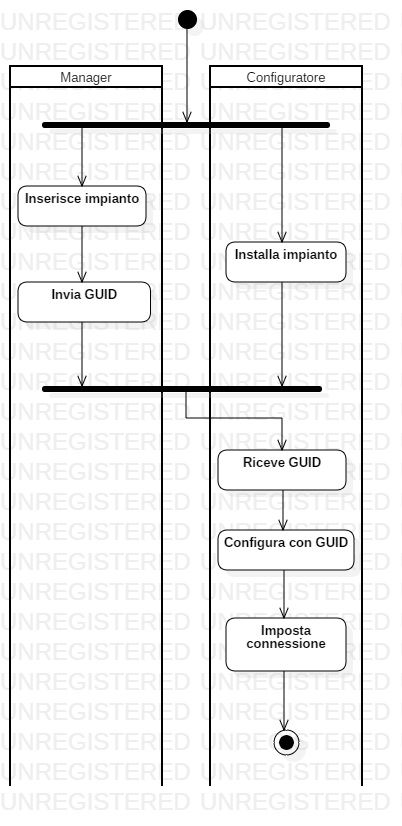
\includegraphics[scale=0.55]{img/activity_registration.png}
  \caption{Processo di registrazione di un nuovo impianto}
\end{figure}
\newpage
%----------------------------------------------------------------------------------------
%	IMPLEMENTAZIONE
%----------------------------------------------------------------------------------------

\section{Implementazione}\label{sec:implementazione}

Esporre i principali problemi affrontati durante l'effettiva realizzazione delle componenti hardware/software e illustrare le soluzioni implementative adottate. Se l'elaborato ha previsto l'utilizzo di tecnologie già disponibili sul mercato, discuterne brevemente le caratteristiche e motivarne l'adozione rispetto ad altre soluzioni assimilabili.\\

\textbf{NOTA: in questa sezione devono essere riportate esclusivamente le porzioni di codice ritenute particolarmente significative. Il codice sorgente nella sua interezza, opportunamente commentato, deve essere consegnato separatamente dalla relazione in un archivio compresso.}\\


Vincoli circa la lunghezza della sezione (escluse didascalie, tabelle, testo nelle immagini, schemi):

\vspace{1cm}
\begin{tabular}{l|rr}
 & Numero minimo di battute & Numero massimo di battute \\
 \hline
 1 componente & 5000 & 11000 \\
 2 componenti & 8000 & 16000 \\
 3 componenti & 10000 & 21000 \\
 \hline
\end{tabular}
\newpage
\subsection{Implementazione parte locale}
\newpage
\subsection{Implementazione parte Applicativa}
\subsubsection{Manager}
\paragraph{Caratteristiche Principali}
Il capitolo di progettazione di \textit{manager} prevedeva lo sviluppo di una applicazione web di tipo SPA caratterizzata da una certa complessità, facilità di manutenzione e scalabilità.\\
Con queste premesse, il team di sviluppo ha deciso di adottare \textit{Angular} come framework per lo sviluppo dell'applicazione.\\\\
Adottato specificatamente nella versione 6+, \textit{Angular} è un set di librerie frontend open-source studiate appostiamente per una creazione agevole e strutturata di SPA; creata e mantenuta tutt'ora direttamente da \textit{Google}, questo framework si posiziona al primo posto per popolarità per la creazione di progetti enterprise web.\\
Benché infatti si presti anche alla creazione di prodotti di ridotta complessità, lo sviluppo attraverso \textit{Angular} è caratterizzato da una curva di apprendimento ripida e dalla necessità di scrivere molto codice \textit{boilerplate} per sviluppare funzionalità semplici; benché queste caratteristiche lo rendano capace di strutturare adeguatamente progetti frontend complessi, molti team di sviluppo lo ritengono uno strumento troppo potente (e difficile) per le loro necessità.\\
Concludendo, questo \textit{framework} è stato scelto rispetto ad altre librerie popolari (come \textit{React} o \textit{Vue}) per i seguenti motivi:
\begin{itemize}
\item \textit{Angular} fornisce direttamente funzionalità utili allo sviluppo di SPA come \textit{Dependency Injection}, \textit{AJAX}, gestione token ecc.\\
I suoi principali competitor, essendo librerie e non \textit{framework}, richiedono l'integrazione con dipendenze di terze parti (esponendo il prodotto a una minore mantenibilità).
\item Grazie a una suddivisione in moduli e sottomoduli e al supporto della \textit{Dependency Injection
}, un applicazione scritta attraverso \textit{Angular} permette di scalare la sua complessità in maniera nettamente migliore rispetto al processo non strutturato e completamente in mano al programmatore tipico delle altre librerie.
\item Avendo già sviluppato prodotti di una certa complessità attraverso questo framework, il team di sviluppo si è dimostrato particolarmente efficiente.
\end{itemize}
L'applicazione è stata scritta in Typescript, super-set di Javascript che permette di scrivere codice per applicazioni web attraverso il paradigma ad oggetti.\\
La sua notevole somiglianza con il linguaggio c\#, inoltre, ha reso lo sviluppo del lato server più semplice (dato che è stato scritto in asp.net core).
\paragraph{Librerie}
Segnaliamo qui le dipendenze esterne degne di nota necessarie al funzionamento del progetto:
\begin{itemize}
\item \textit{Angular Material:} libreria per interfacce utente basate sul \textit{material design} e largamente supportata dalla comunità dell'omonimo \textit{framework}.\\
Gran parte degli artefatti grafici presente nell'applicazione (tabelle, notifiche, inputs) sono disegnati grazie all'utilizzo di questa versatile libreria.
\item \textit{Ngx local storage:} libreria che consente di archiviare valori nella cache del browser attraverso una serie di strategie (indexedDB, local storage ecc.).\\
Viene unicamente utilizzata per mantenere in memoria il \textit{loginToken}.
\end{itemize}
\paragraph{Codice}
In \textit{Angular}, ogni componente visiva principale dell'applicazione viene modellata come un \textit{Component}, cioè un costrutto composto da un \textit{controller} (cioè una parte nella quale risiede la logica del componente: funzioni, variabili, hooks) e un \textit{template} (cioè, in ambito web, un sezione di HTML e CSS).\\
Questo elemento è indispensabile per specificare singole funzionalità o parti riusabili dell'applicazione, grazie alla sua sintassi precisa e inedita nel mondo dello sviluppo frontend.\\
Considerato inoltre che i progetti \textit{Angular} devono passare attraverso una procedura di compilazione (o, più precisamente, transpilazione) dei sorgenti, si può capire come lo sviluppo di applicazioni particolarmente complesse venga agevolata: ogni file sarà esente da errori di compilazione (anche grazie all'uso del paradigma OOP) e il progetto avrà una struttura chiara e definita formalmente.
\newpage
Come primo esempio viene presentato il \textit{component} dedito alla login utente:
\begin{lstlisting}

import { Component } from '@angular/core';
@Component({
  selector: 'app-login',
  templateUrl: './login.component.html',
  styleUrls: ['./login.component.scss']
})
export class LoginComponent {
// constructor(loginService: LoginService...) {}

  login(form: NgForm) {
    this.loginService.login(form.v.username, form.v.password).subscribe(success => {     
     
        if (success) 
          this.router.navigate(['']);
        else
          this.snack.open("Wrong username or password", null, {panelClass: 'loginSnackbar'});
    });
  }}
\end{lstlisting}
\phantom{\\}
Si possono notare i seguenti punti d'interesse: 
\begin{itemize}
\item Importazione delle dipendenze attraverso la parola chiave \textit{import}.\\
Questo meccanismo si può considerare simile all'inclusione di package presente in C\# e Java.
\item Dichiarazione del componente attraverso il decoratore \textit{@Component}.\\ 
Un decoratore non è altro che un meccanismo per estendere le funzionalità di una classe attraverso il framework.
\item Subscription del form di login: ogni tentativo di login da parte dell'utente richiamerà la lambda mostrata.\\
In caso di successo, viene spostata la navigazione utente alla home della webApp.\\
In caso contrario, viene mostrata una notifica di errore grazie alla libreria \textit{Angular Material}.
\end{itemize}
Un altra sezione di particolare interesse sono le \textit{Routes} e le \textit{Guards}.\\
Le prime vengono utilizzate dal framework per impostare gli url a cui l'applicazione dovrà rispondere: attraverso di esse sarà possibile specificare quale \textit{Component} mostrare e con quali parametri.\\
Le seconde, invece, possono essere associate a \textit{routes} per determinare la loro attivazione in base alle condizioni inserite: \textit{manager} utilizza delle \textit{guards} per prevenire che utenti non autenticati possano accedere a sezioni protette dell'applicazione.\\\\
Un esempio di tale guard viene presentata di seguito:
\begin{lstlisting}

import { Injectable } from "@angular/core";
@Injectable()
export class AuthGuard implements CanActivate {
//  constructor(storage: LocalStorage...) {}

    canActivate() {
        if (!this.loginService.user == null)
            return true;

        return this.storage.getItem('loginToken').
        pipe(concatMap(loginToken => {
            if (loginToken == null) {
                this.router.navigate(['/login']);
                return of(false);
            }
            return this.loginService.loginByToken(loginToken);
        }));
    }
}
\end{lstlisting}
Anche qui vengono evidenziati i seguenti punti d'interesse:
\begin{itemize}
\item In modo analogo al componente descritto in precedenza, in questa classe viene specificato un decoratore (\textit{@Injectable}) per donare alla classe uno specifico comportamento.
\item L'implementazione dell'interfaccia \textit{CanActivate} serve a specificare la tipologia di \textit{Guard} che verrà implementata: in questo caso si tratterà della più semplice, cioè per determinare se attivare o no una certa \textit{Route} richiesta (attraverso il metodo \textit{canActivate()}.
\item \textit{this.storage.getItem()} rappresenta è un esempio di utilizzo della libreria \textit{Ngx local storage} descritta nella sezione precedente: in questo caso mostrato il reperimento di un \textit{loginToken} di sessione.\\
Qualora il token non esista (e quindi l'utente non sia autenticato) allora si rimanda l'applicazione all'indirizzo di login.\\
In caso contrario la \textit{Route} viene accettata e fatta proseguire.
\end{itemize}
\newpage
\subsubsection{Consumer}
\paragraph{Caratteristiche Principali}
Il capitolo di progettazione di \textit{consumer} evidenzia la necessità di sviluppare \textit{consumer} come un'applicazione di tipo PWA.\\
Questa scelta è stata dovuta principalmente ai suoi più rapidi tempi di sviluppo rispetto a una normale app nativa; date le ridotte risorse a disposizione, il team di sviluppo è sempre stato propenso a ridurre i costi, dove possibile.\\
Pertanto, per evitare di investire tempo nella formazione di personale per l'utilizzo di tecnologie specifiche per PWA, è stato deciso di utilizzare \textit{Angular} per lo sviluppo di \textit{Consumer}.\\\\
La natura poliedrica di questo framework, infatti, permette di aggiungere il supporto alle \textit{Progressive Web apps} attraverso dei semplici moduli e pochi file di configurazione aggiuntivi: gran parte del funzionamento dell'app, infatti, verrà gestita da \textit{Angular} (ad esempio, non sarà necessario sviluppare direttamente un \textit{service worker}).\\
Infine, anche in questo caso verrà utilizzato \textit{Typescript} come linguaggio di programmazione
\paragraph{Librerie}

Segnaliamo qui le dipendenze esterne degne di nota necessarie al funzionamento del progetto:
\begin{itemize}
\item \textit{Angular Material:} anche in questo caso è stata utilizzata questa libreria per il disegno e la gestione delle interfacce utente.\\
Utilizzare la stessa dipendenza nei due prodotti si è dimostrato utile nel risparmiare sui costi di sviluppo, dato che la tecnologia adottata era divenuta familiare.
\item \textit{Angular Google Maps Core:} i requisiti esposti dal committente rendono chiaro il desiderio di mostrare una \textit{gmap} per orientare l'utente nella ricerca di un bagno pubblico; ciò è stato possibile grazie all'inclusione della libreria \textit{Angular Google Maps Core} all'interno del progetto.\\
Per poter avviare il servizio, inoltre, è stato necessario fornire all'applicazione un apposita chiave di identificazione.

\end{itemize}
\paragraph{Codice}
Dato il suo sviluppo in \textit{Angular} come il già analizzato \textit{manager}, non verranno qua analizzate le modalità di costruzione delle funzionalità di \textit{consumer}, che si possono infatti considerare pressoché simili.\\
Inoltre, dato che gran parte del codice necessario per rendere \textit{consumer} una PWA non è stato sviluppato direttamente dal team ma generato automaticamente dal framework (attraverso un tool di transpilazione chiamato \textit{angular-cli}) non si ritiene meritevole di interesse il suo approfondimento.\\\\
Tuttavia, si ritiene importante approfondire le modalità con le quali è stato possibile mostrare a schermo una \textit{gmap} interattiva con l'utente, in particolare il lato \textit{template} che è stato tralasciato nella precedente sezione.\\
Innanzitutto, \textit{Angular} consente di effettuare un \textit{binding} (cioè un collegamento) tra una variabile presente nel \textit{controller} e il rispettivo \textit{template} attraverso due modalità: \textit{box casing} (cioè racchiudendo l'attributo a cui assegnare una variabile tramite i caratteri []) oppure tramite \textit{double brackets} (cioè racchiudere il nome della variabile assegnata a un certo attributo tramite i caratteri \{\}).\\\\
Ad esempio, l'implementazione della \textit{gmap} nel componente è stato effettuato attraverso un binding di tipo \textit{box casing}, come mostrato di seguito: 
\begin{lstlisting}[style=htmlcssjs]

<agm-map [latitude]="userPosition[0]" [longitude]="userPosition[1]"
[zoom]="14">

  <agm-marker *ngFor="let restRoom of restRooms; let i = index"
              (markerClick)="restRoomSelected(restRoom)"
              [latitude]="restRoom.address[0]"
              [longitude]="restRoom.address[1]">

    <agm-info-window>
      <app-marker-detail [restRoom]="restRoom"></app-marker-detail>
    </agm-info-window>
  </agm-marker>
</agm-map>
\end{lstlisting}
\newpage
Oltre al \textit{binding}, si possono notare i seguenti punti d'interesse:
\begin{itemize}
	\item \textit{agm-map}, \textit{agm-marker} e \textit{agm-info-window} sono componenti esterni forniti dalla libreria \textit{Angular Material}.\\ Come qualsiasi altro elemento HTML, possono essere  istanziati semplicemente specificando il loro nome nel template. 
	\item Il componente \textit{agm-marker} viene istanziato tante volte quanti sono gli elementi presenti nell'array \textit{restRooms} del \textit{controller} (grazie alla direttiva \textit{*ngFor}).\\ Visivamente, ciò permette di disegnare i \textit{marker} descritti nell'analisi dei requisiti e mostrati nel mockup della fase di progettazione.
	\item \textit{app-marker-detail} invece corrisponde a un componente scritto dal team di sviluppo: esso servirà a rappresentare il contenuto esposto (\textit{popover}) al click di un marker.
\end{itemize}
\newpage
\subsection{Implementazione parte centrale}
\subsubsection{Server}
\paragraph{Caratteristiche}
La progettazione della parte centrale del sistema ha previsto la creazione di un generico server RESTFul in grado di rispondere alle richieste delle altre entità coinvolte nel sistema.\\
Dato che i requisti del committente non hanno dato alcuna indicazione sul suo ambiente di destinazione e la progettazione non ha individuato vincoli in tal senso, il team di sviluppo ha optato per una soluzione multipiattaforma, gratuita e opensource come \textit{ASP.NET Core}.\\
Questo framework di sviluppo backend è stato creato e tutt'ora direttamente mantenuto da \textit{Microsoft}, in futura sostituzione del più classico ambiente ASP.NET; dalla sua introduzione (circa 2016) ha ricevuto una crescente popolarità come soluzione general-purpose backend.\\
Comunque, le motivazioni che hanno spinto il team di sviluppo a scegliere questa tecnologia possono essere così riassunte: 
\begin{itemize}
\item Le elevate prestazioni garantite dal framework (sopratutto in situazioni di elevato carico da parte di host multipli) lo rendono perfettamente adatto al carico di lavoro previsto del progetto.
\item La natura multipiattaforma di \textit{ASP.NET Core} consente una notevole flessibilità sull'ambiente di hosting di destinazione.\\
Ciò consentirà una scelta più ampia e concorrenziale e, pertanto, un maggiore ritorno economico del sistema.
\item La stretta vicinanza con l'ambiente di sviluppo delle applicazioni frontend (scritte in Typescript) ha migliorato l'efficienza generale del team.\\
Data la notevole somiglianza dei linguaggi C\# e Typescript, infatti, non è stato necessario assegnare risorse nella formazione degli sviluppatori.
\end{itemize}

\subsubsection{DBMS}
\paragraph{Caratteristiche Principali}
\newpage



%----------------------------------------------------------------------------------------
%	TESTING E PERFORMANCE
%----------------------------------------------------------------------------------------

\section{Testing e performance}

Esporre lo stato di funzionamento effettivo del sistema progettato ad elaborato concluso. Per ciascuna delle funzionalità salienti devono essere tabellate e discusse le performance riscontrate mediante opportuni test eseguiti in fase di validazione del progetto.\\

I tempi di esecuzione/comunicazione devono essere accompagnati dalle caratteristiche dell'hardware sul quale è eseguito il software.\\

Qualora l'elaborato includa algoritmi innovativi, indicarne la complessità computazionale (avendo cura di esporre lo pseudo codice nella sezione \ref{sec:implementazione}).\\


Vincoli circa la lunghezza della sezione (escluse didascalie, tabelle, testo nelle immagini, schemi):

\vspace{1cm}
\begin{tabular}{l|rr}
 & Numero minimo di battute & Numero massimo di battute \\
 \hline
 1 componente & 2000 & 3000 \\
 2 componenti & 2500 & 4500 \\
 3 componenti & 3000 & 6000 \\
 \hline
\end{tabular}


\newpage


%----------------------------------------------------------------------------------------
%	ANALISI DI DEPLOYMENT SU LARGA SCALA
%----------------------------------------------------------------------------------------

\section{Analisi di deployment su larga scala}

In questa sezione va discussa, eventualmente con l'ausilio di opportuni diagrammi (componenti, deployment), l'evoluzione del progetto presentato immaginando che venga adottato su larga scala. I dettagli qui esposti devono quindi astrarre dalle specifiche dell'elaborato qualora l'implementazione sia stata focalizzata su uno scenario isolato.\\

A titolo d’esempio, qualora applicabile, devono essere evidenziate le criticità che si potrebbero incontrare e devono essere proposte soluzioni tipiche in contesti di \textit{cloud architecture} per garantire un'adeguata \textit{resilienza}, in termini di \textit{availability} e \textit{scalability} del sistema.\\


Vincoli circa la lunghezza della sezione (escluse didascalie, tabelle, testo nelle immagini, schemi):

\vspace{1cm}
\begin{tabular}{l|rr}
 & Numero minimo di battute & Numero massimo di battute \\
 \hline
 1 componente & 3000 & 6000 \\
 2 componenti & 4500 & 9000 \\
 3 componenti & 6000 & 12000 \\
 \hline
\end{tabular}


\newpage


%----------------------------------------------------------------------------------------
%	PIANO DI LAVORO
%----------------------------------------------------------------------------------------

\section{Piano di lavoro}

In questa sezione devono essere chiariti i compiti svolti da ciascun candidato nel caso in cui il gruppo abbia più di un componente.\\

Deve essere inoltre esposto il piano di lavoro adottato. A tal fine, per ogni attività svolta durante la preparazione dell'elaborato (ad esempio: studio di una tecnologia, progettazione di un componente, implementazione di un algoritmo ecc…) deve essere chiarita la collocazione temporale e devono essere indicate le risorse impiegate per svolgerla (giorni/uomo). I candidati possono ricorrere a opportuni diagrammi come quello di Gantt.\\


Vincoli circa la lunghezza della sezione (escluse didascalie, tabelle, testo nelle immagini, schemi):

\vspace{1cm}
\begin{tabular}{l|rr}
 & Numero minimo di battute & Numero massimo di battute \\
 \hline
 1 componente & 1000 & 2000 \\
 2 componenti & 1500 & 3000 \\
 3 componenti & 2000 & 4000 \\
 \hline
\end{tabular}

\newpage


%----------------------------------------------------------------------------------------
%	CONCLUSIONI
%----------------------------------------------------------------------------------------

\section{Conclusioni}

Esporre brevemente le considerazioni conclusive sul progetto presentato, indicando anche i possibili sviluppi futuri.\\

Vincoli circa la lunghezza della sezione (escluse didascalie, tabelle, testo nelle immagini, schemi):

\vspace{1cm}
\begin{tabular}{l|rr}
 & Numero minimo di battute & Numero massimo di battute \\
 \hline
 1 componente & 500 & 1000 \\
 2 componenti & 1000 & 2000 \\
 3 componenti & 1500 & 3000 \\
 \hline
\end{tabular}

\newpage


%----------------------------------------------------------------------------------------
%	APPENDICE
%----------------------------------------------------------------------------------------

\appendix
\addcontentsline{toc}{section}{Appendice}
\section*{Appendice}
Laddove necessario è possibile avvalersi di appendici alla relazione per includere materiale di approfondimento.\\

A titolo esemplificativo possono essere incluse le schede tecniche dei componenti adottati, la normativa di riferimento che regola un particolare dominio applicativo, ecc.


\newpage


%----------------------------------------------------------------------------------------
%	RIFERIMENTI BIBLIOGRAFICI
%----------------------------------------------------------------------------------------
\addcontentsline{toc}{section}{Riferimenti bibliografici}
\begin{thebibliography}
EElencare i riferimenti bibliografici citati nel testo. 
\end{thebibliography}

%----------------------------------------------------------------------------------------

\end{document}